%%%%%%%%%%%%%%%%%%%%%%%%%%%%%%%%%%%%%%%%%
% Programming/Coding Assignment
% LaTeX Template
%
% This template has been downloaded from:
% http://www.latextemplates.com
%
% Original author:
% Ted Pavlic (http://www.tedpavlic.com)
%
% Note:
% The \lipsum[#] commands throughout this template generate dummy text
% to fill the template out. These commands should all be removed when 
% writing assignment content.
%
% This template uses a Perl script as an example snippet of code, most other
% languages are also usable. Configure them in the "CODE INCLUSION 
% CONFIGURATION" section.
%
%%%%%%%%%%%%%%%%%%%%%%%%%%%%%%%%%%%%%%%%%

%----------------------------------------------------------------------------------------
%	PACKAGES AND OTHER DOCUMENT CONFIGURATIONS
%----------------------------------------------------------------------------------------

\documentclass{article}

\usepackage{fancyhdr} % Required for custom headers
\usepackage{lastpage} % Required to determine the last page for the footer
\usepackage{extramarks} % Required for headers and footers
\usepackage[usenames,dvipsnames]{color} % Required for custom colors
\usepackage{graphicx} % Required to insert images
\usepackage{subcaption}
\usepackage{listings} % Required for insertion of code
\usepackage{courier} % Required for the courier font
\usepackage{lipsum} % Used for inserting dummy 'Lorem ipsum' text into the template
\usepackage{url}
\newcommand{\quotes}[1]{``#1''}
% Margins
\topmargin=-0.45in
\evensidemargin=0in
\oddsidemargin=0in
\textwidth=6.5in
\textheight=9.0in
\headsep=0.25in

\linespread{1.1} % Line spacing

% Set up the header and footer
\pagestyle{fancy}
\lhead{\hmwkAuthorName} % Top left header
\chead{\hmwkClass\ (\hmwkClassInstructor\ \hmwkClassTime) \hmwkTitle} % Top center head
\rhead{\firstxmark} % Top right header
\lfoot{\lastxmark} % Bottom left footer
\cfoot{} % Bottom center footer
\rfoot{Page\ \thepage\ of\ \protect\pageref{LastPage}} % Bottom right footer
\renewcommand\headrulewidth{0.4pt} % Size of the header rule
\renewcommand\footrulewidth{0.4pt} % Size of the footer rule

\setlength\parindent{0pt} % Removes all indentation from paragraphs

%----------------------------------------------------------------------------------------
%	CODE INCLUSION CONFIGURATION
%----------------------------------------------------------------------------------------

\definecolor{MyDarkGreen}{rgb}{0.0,0.4,0.0} % This is the color used for comments
\lstloadlanguages{R} % Load Perl syntax for listings, for a list of other languages supported see: ftp://ftp.tex.ac.uk/tex-archive/macros/latex/contrib/listings/listings.pdf
\lstset{language=R, % Use Perl in this example
        frame=single, % Single frame around code
        basicstyle=\small\ttfamily, % Use small true type font
        keywordstyle=[1]\color{Blue}\bf, % Perl functions bold and blue
        keywordstyle=[2]\color{Purple}, % Perl function arguments purple
        keywordstyle=[3]\color{Blue}\underbar, % Custom functions underlined and blue
        identifierstyle=, % Nothing special about identifiers                                         
        commentstyle=\usefont{T1}{pcr}{m}{sl}\color{MyDarkGreen}\small, % Comments small dark green courier font
        stringstyle=\color{Purple}, % Strings are purple
        showstringspaces=false, % Don't put marks in string spaces
        tabsize=5, % 5 spaces per tab
        %
        % Put standard Perl functions not included in the default language here
        morekeywords={},
        %
        % Put Perl function parameters here
        morekeywords=[2]{on, off, interp},
        %
        % Put user defined functions here
        morekeywords=[3]{test},
       	%
        morecomment=[l][\color{Blue}]{...}, % Line continuation (...) like blue comment
        numbers=left, % Line numbers on left
        firstnumber=1, % Line numbers start with line 1
        numberstyle=\tiny\color{Blue}, % Line numbers are blue and small
        stepnumber=5 % Line numbers go in steps of 5
}

% Creates a new command to include a perl script, the first parameter is the filename of the script (without .pl), the second parameter is the caption
\newcommand{\rscript}[2]{
\begin{itemize}
\item[]\lstinputlisting[caption=#2,label=#2]{#1.R}
\end{itemize}
}

%----------------------------------------------------------------------------------------
%	DOCUMENT STRUCTURE COMMANDS
%	Skip this unless you know what you're doing
%----------------------------------------------------------------------------------------

% Header and footer for when a page split occurs within a problem environment
\newcommand{\enterProblemHeader}[1]{
\nobreak\extramarks{#1}{#1 continued on next page\ldots}\nobreak
\nobreak\extramarks{#1 (continued)}{#1 continued on next page\ldots}\nobreak
}

% Header and footer for when a page split occurs between problem environments
\newcommand{\exitProblemHeader}[1]{
\nobreak\extramarks{#1 (continued)}{#1 continued on next page\ldots}\nobreak
\nobreak\extramarks{#1}{}\nobreak
}

\setcounter{secnumdepth}{0} % Removes default section numbers
\newcounter{homeworkProblemCounter} % Creates a counter to keep track of the number of problems

\newcommand{\homeworkProblemName}{}
\newenvironment{homeworkProblem}[1][Problem \arabic{homeworkProblemCounter}]{ % Makes a new environment called homeworkProblem which takes 1 argument (custom name) but the default is "Problem #"
\stepcounter{homeworkProblemCounter} % Increase counter for number of problems
\renewcommand{\homeworkProblemName}{#1} % Assign \homeworkProblemName the name of the problem
\section{\homeworkProblemName} % Make a section in the document with the custom problem count
\enterProblemHeader{\homeworkProblemName} % Header and footer within the environment
}{
\exitProblemHeader{\homeworkProblemName} % Header and footer after the environment
}

\newcommand{\problemAnswer}[1]{ % Defines the problem answer command with the content as the only argument
\noindent\framebox[\columnwidth][c]{\begin{minipage}{0.98\columnwidth}#1\end{minipage}} % Makes the box around the problem answer and puts the content inside
}

\newcommand{\homeworkSectionName}{}
\newenvironment{homeworkSection}[1]{ % New environment for sections within homework problems, takes 1 argument - the name of the section
\renewcommand{\homeworkSectionName}{#1} % Assign \homeworkSectionName to the name of the section from the environment argument
\subsection{\homeworkSectionName} % Make a subsection with the custom name of the subsection
\enterProblemHeader{\homeworkProblemName\ [\homeworkSectionName]} % Header and footer within the environment
}{
\enterProblemHeader{\homeworkProblemName} % Header and footer after the environment
}

%----------------------------------------------------------------------------------------
%	NAME AND CLASS SECTION
%----------------------------------------------------------------------------------------

\newcommand{\hmwkTitle}{Homework\ \#2} % Assignment title
\newcommand{\hmwkDueDate}{Sunday, Feb 9,  2018 10:00 p.m.}% Due date
\newcommand{\hmwkClass}{Introduction to Data Analysis and Mining\\} % Course/class
\newcommand{\hmwkClassTime}{} % Class/lecture time
\newcommand{\hmwkClassInstructor}{Instructor: Hasan Kurban} % Teacher/lecturer
\newcommand{\hmwkAuthorName}{Kwong Yuet Michael Fadillah Wong} % Your name

%----------------------------------------------------------------------------------------
%	TITLE PAGE
%----------------------------------------------------------------------------------------

\title{
\vspace{2in}
\textmd{\textbf{\hmwkClass\ \hmwkTitle}}\\
\normalsize\vspace{0.1in}\small{Due\ on\ \hmwkDueDate}\\
\vspace{0.1in}\large{\textit{\hmwkClassInstructor\ }}
\vspace{3in}
}

\author{\textbf{\hmwkAuthorName}}
\date{\today} % Insert date here if you want it to appear below your name

%----------------------------------------------------------------------------------------

\begin{document}


\maketitle

%----------------------------------------------------------------------------------------
%	TABLE OF CONTENTS
%----------------------------------------------------------------------------------------

%\setcounter{tocdepth}{1} % Uncomment this line if you don't want subsections listed in the ToC

\newpage
\tableofcontents
\newpage

%----------------------------------------------------------------------------------------
%	PROBLEM 1
%----------------------------------------------------------------------------------------

\begin{homeworkProblem} 

Textbook exercises, chapter 2, pages: 91-93
\begin{enumerate}
\item Exercise 12  \textbf{(10 points)}\\
12a) Noise is not interesting nor desirable, and outlier is interesting and desirable.\\
12b) Yes, Noise can be outlier\\
12c) No, Noise is not always outlier, it can also modifies the data object.\\
12d) No, it can be the one class that is different than other attributes.\\
12e) Yes
\item Exercise 15  \textbf{(10 points)}\\
15a) We select n*mi/m elements from the group\\
15b) We view all the data as a whole, and select n elements from the data.\\
\item Exercise 16  \textbf{(10 points)}\\
16a) For one document, terms have max weight, while terms have 0 weight in every document.\\
16b) From this transformation, terms occur in every document cannot individualize one document from another.
\item Exercise 18  \textbf{(15 points)}\\
18a) Hamming distance = 3\\
Jaccard Similarity = 2/5 = 0.4\\
18b) Hamming distance is more similar to the Simple Matching Coefficient, because Simple Matching Coefficient = Hamming distance / number of bits.\\
The Jaccard similarity is more similar to the cosine measure, becuase they ignore matches.\\
18c) Jaccard similarity, because we want to see the number matches.\\
18d) Hamming distance, because we need to find the difference between genes in order to compare the genetic makeup of two organisms of the same species.
\item Exercise 19  \textbf{(15 points)}\\
19a) 
Correlation:$> cor(c(1,1,1,1),c(2,2,2,2))$\\
$[1] NA$\\
Euclidean distance:$> sqrt(sum((c(1,1,1,1)-c(2,2,2,2))^2))$\\
$[1] 2$\\
cos:(8/(2*4)) = 1\\
19b) 
Correlation:$> cor(c(0,1,0,1),c(1,0,1,0))$\\
$[1] -1$\\
Euclidean distance:$> sqrt(sum((c(0,1,0,1)-c(1,0,1,0))^2))$\\
$[1] 2$\\
Jaccard: number of matches = 0.\\
Therefore Jaccard Similarity = 0\\
cos: numerator = 0, cosine similarity = 0\\
19c) 
Correlation:$> cor(c(0,-1,0,1),c(1,0,-1,0))$\\
$[1] 0$\\
Euclidean distance:$> sqrt(sum((c(0,-1,0,1)-c(1,0,-1,0))^2))$\\
$[1] 2$\\
cos: numerator = 0, cosine similarity = 0\\
19d) 
Correlation:$> cor(c(1,1,0,1,0,1),c(1,1,1,0,0,1))$\\
$[1] 0.25$\\
Jaccard: 3/(6-1) = 0.6\\
cos: (3/(2*2)) = 3/4 = 0.75\\
19e)
Correlation:$> cor(c(2,−1, 0, 2, 0,−3),c(−1, 1,−1, 0, 0,−1))$\\
$[1] 0$\\
cos: numerator = -2 -1 + 3 = 0, cosine similarity = 0
\end{enumerate}
\end{homeworkProblem}



%----------------------------------------------------------------------------------------
%	PROBLEM 2
%----------------------------------------------------------------------------------------

% To have just one problem per page, simply put a \clearpage after each problem


\begin{homeworkProblem} 
For the following data, give the best taxonomic type (interval, ratio, nominal, ordinal):
\begin{enumerate}
\item A section of highway on a map.\\
Nominal
\item The value of a stock.\\
Interval
\item The weight of a person.\\
Ratio
\item Marital status.\\
Nominal
\item Visiting United Airlines (\url{https://www.united.com}) the seating is: Economony, Economy plus, and United Business.  \textbf{(10 points: each question is worth 2 points)}\\
Ordinal
\end{enumerate}
\end{homeworkProblem}

%----------------------------------------------------------------------------------------
%	PROBLEM 3
%----------------------------------------------------------------------------------------


\begin{homeworkProblem}
You are datamining with a column that has physical addresses in some city with the same zipcode.  For example,
\begin{verbatim}

55 WEST CIR
2131 South Creek Road
Apt. #1 Fountain Park
1114 Rosewood Cir
1114 Rosewood Ct.
1114 Rosewood Drive

\end{verbatim}

What structure would you create to mine these?  What questions do you think you should be able to answer?  \textbf{(10 points)}\\
I will divide the address into three parts; apartment number, street name, and street suffix. For example:\\
For 2131 South Creek Road:\\
Apartment number: 2131\\
Street name: South Creek\\
Street Suffix: Road\\
By this kind of structure, we can answer the address by part, such as how common is the street name overlapped?
\end{homeworkProblem}

%----------------------------------------------------------------------------------------
%	PROBLEM 3
%----------------------------------------------------------------------------------------


\begin{homeworkProblem}
The Wisconsin Breast Cancer data set is very famous. Here is the URL \url{https://archive.ics.uci.edu/ml/datasets/breast+cancer+wisconsin+(original)}.  In the Data Folder are multiple files.  Here is the beginning of an R session that allows us to read this data from the web into our local R session:
\begin{verbatim}
> install.packages("data.table")
> library(data.table)
> install.packages("curl")
> mydata <- fread("https://archive.ics.uci.edu/ml/machine-learning-databases/
                   breast-cancer-wisconsin/breast-cancer-wisconsin.data")
> head(mydata)
        V1 V2 V3 V4 V5 V6 V7 V8 V9 V10 V11
1: 1000025  5  1  1  1  2  1  3  1   1   2
2: 1002945  5  4  4  5  7 10  3  2   1   2
3: 1015425  3  1  1  1  2  2  3  1   1   2
4: 1016277  6  8  8  1  3  4  3  7   1   2
5: 1017023  4  1  1  3  2  1  3  1   1   2
6: 1017122  8 10 10  8  7 10  9  7   1   4
> 
\end{verbatim}
\subsection{Discussion of Data}
Briefly describe this data set--what is its purpose?  How should it be used? What are the kinds of data it's using?\\
The wisconsin breast cancer data table that examines how a factor responsible to a benign/malicient tumor.\\
We have eleven attributes: id, Clump thickness, uniformity of cell size, uniformity of cell shape, marginal adhesion, single epithelial cell size
bare nuclei, bland chromatin, normal nucleoli, mitoses, amd class.\\
We can transfrom the data into a numeric table since most of the data attributes is shown in a rank (1-10)\\
\subsection{R Code}
 Using R, show code that answers the following questions:
\begin{enumerate} 
\item How many entries are in the data set? Answer here $\ldots$
\begin{lstlisting}
> nrow(mydata)
[1] 699
> nrow(mydata)*11
[1] 7689
\end{lstlisting}
\item How many unknown or missing data are in the data set? Answer here $\ldots$
\begin{lstlisting}
> sum(is.na(mydata))
[1] 16
\end{lstlisting}
\item How many malignant and benign identifiers are there? Answere here $\ldots$
\begin{lstlisting}
> benign <- nrow(mydata[mydata$V11 == 2,])
> benign
[1] 458
> malignant <- nrow(mydata[mydata$V11 == 4,])
> malignant
[1] 241
\end{lstlisting}
\item Make a histogram of each attribute and discuss the distribution of values \textit{e.g.}, are uniform, skewed, normal.  Place images of these histograms into the document.   Show the R code that you used below and discussion below that. 
\begin{lstlisting}
id <- mydata$V1
hist(id)

clumpThinkness <- mydata$V2
hist(clumpThinkness)

uniformityOfCellSize <- mydata$V3
hist(uniformityOfCellSize)

uniformityOfCellShape <- mydata$V4
hist(uniformityOfCellShape)

marginalAdhesion <- mydata$V5
hist(marginalAdhesion)

SingleEpithelialCellSize <- mydata$V6
hist(SingleEpithelialCellSize)

bareNuclei <- mydata$V7
hist(bareNuclei)

blandChromatin <- mydata$V8
hist(blandChromatin)

normalNucleoli <- mydata$V9
hist(normalNucleoli)

mitoses <- mydata$V10
hist(mitoses)

dataClass <- mydata$V11
hist(dataClass)
\end{lstlisting}

\subsection{Discussion of Attributes}
Answer here$\ldots$
For v1 histogram, it can be ignored. Because v1 represent the ID.\\
From v2 to v10 histograms, those graphs show the frequencies of each topic occurrence.\\
For v11 histogram, the data separate into two columns, which are 2 and 4. 2 stands for benign, and 4 stands for malignant. 
\subsection{Histograms}
Place images here with suitable captions.\\
\begin{figure}
  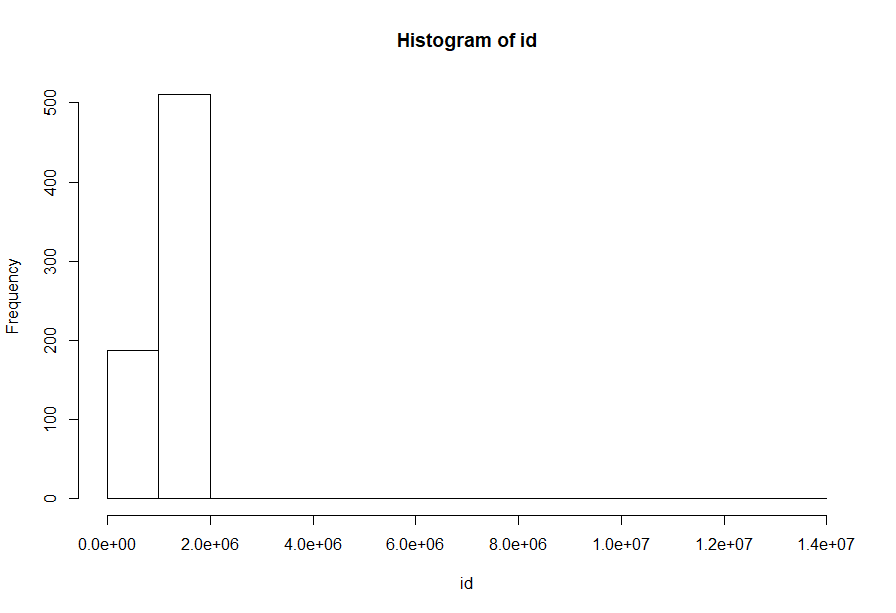
\includegraphics[width=\linewidth]{histv1.png}
  \caption{ID}
\end{figure}
\begin{figure}
  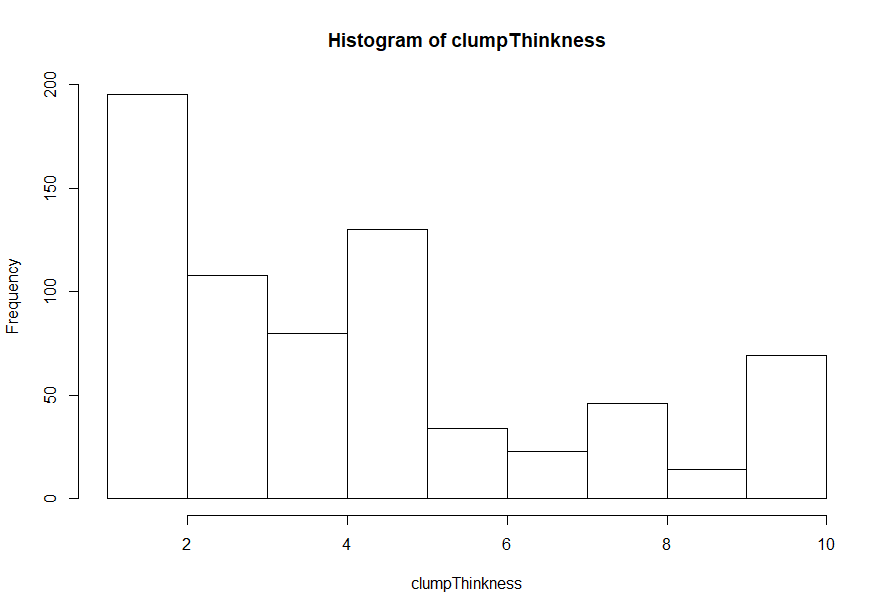
\includegraphics[width=\linewidth]{histv2.png}
  \caption{Clump Thickness}
\end{figure}
\begin{figure}
  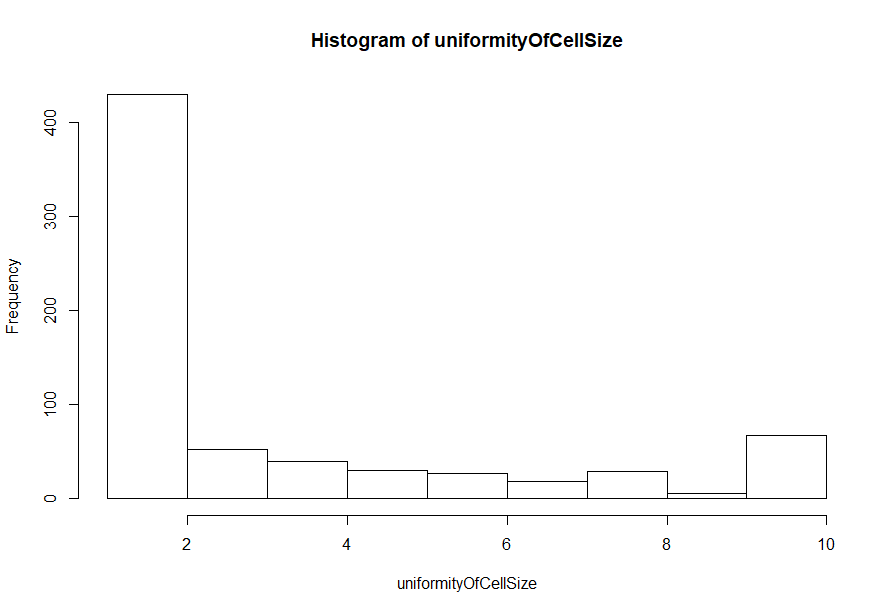
\includegraphics[width=\linewidth]{histv3.png}
  \caption{Uniformity of Cell Size: 1 - 10}
\end{figure}
\begin{figure}
  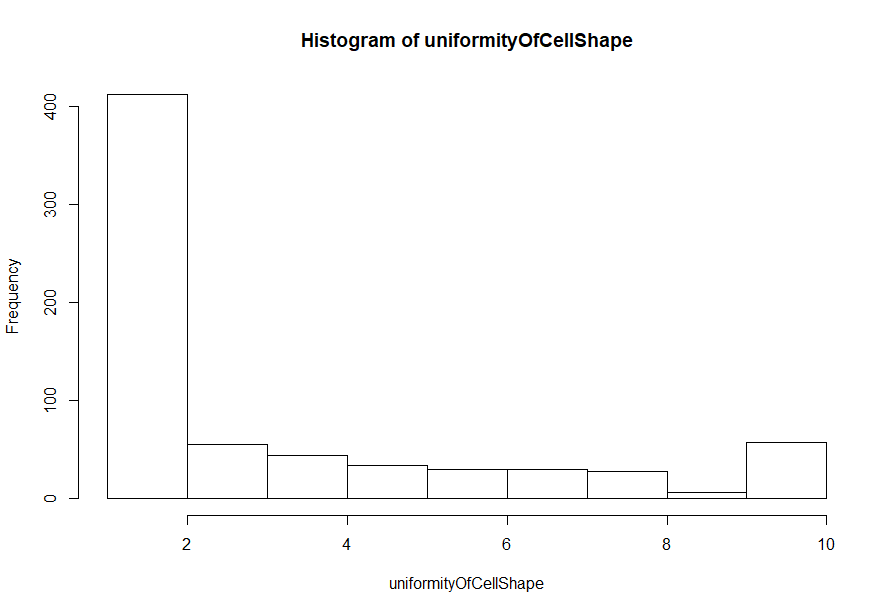
\includegraphics[width=\linewidth]{histv4.png}
  \caption{Uniformity of Cell Shape: 1 - 10}
\end{figure}
\begin{figure}
  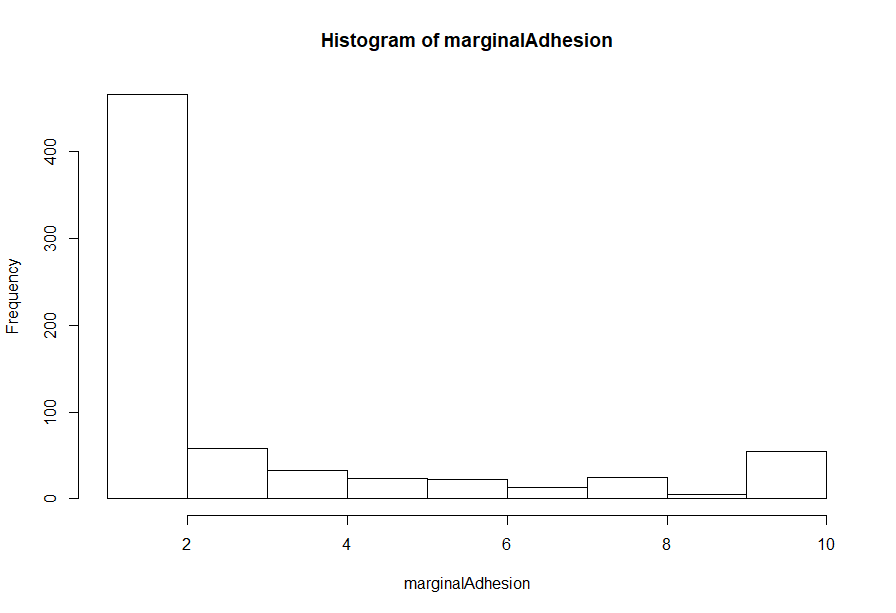
\includegraphics[width=\linewidth]{histv5.png}
  \caption{Marginal Adhesion: 1 - 10}
\end{figure}
\begin{figure}
  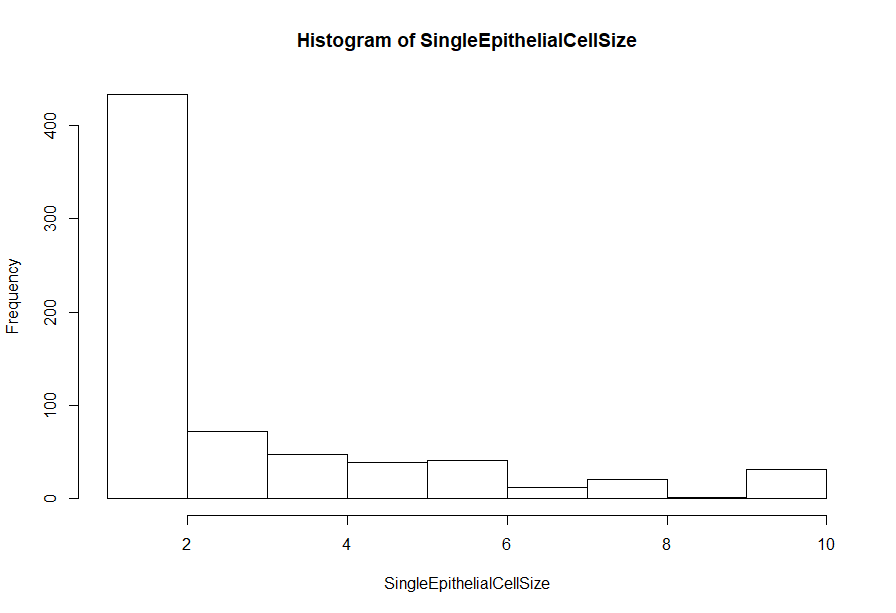
\includegraphics[width=\linewidth]{histv6.png}
  \caption{Single Epithelial Cell Size: 1 - 10}
\end{figure}
\begin{figure}
  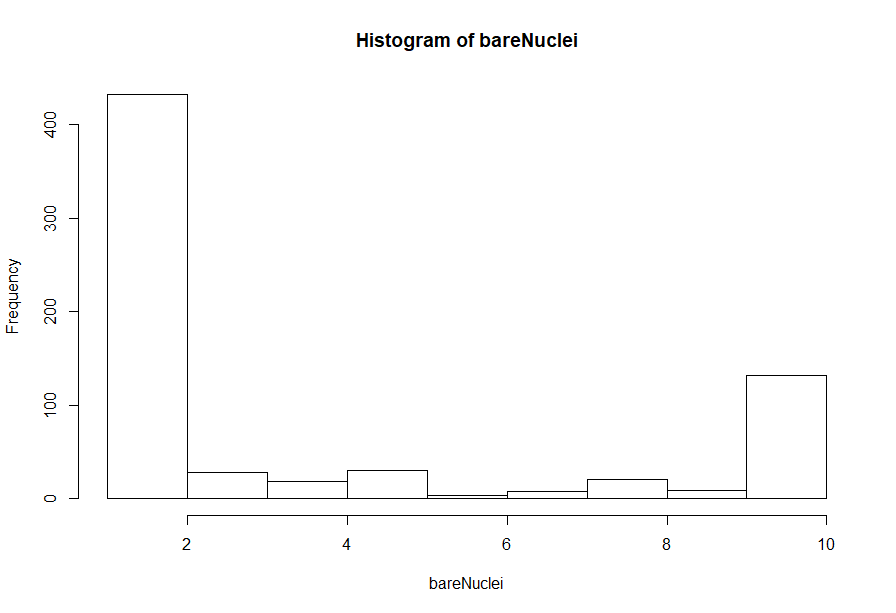
\includegraphics[width=\linewidth]{histv7.png}
  \caption{Bare Nuclei: 1 - 10}
\end{figure}
\begin{figure}
  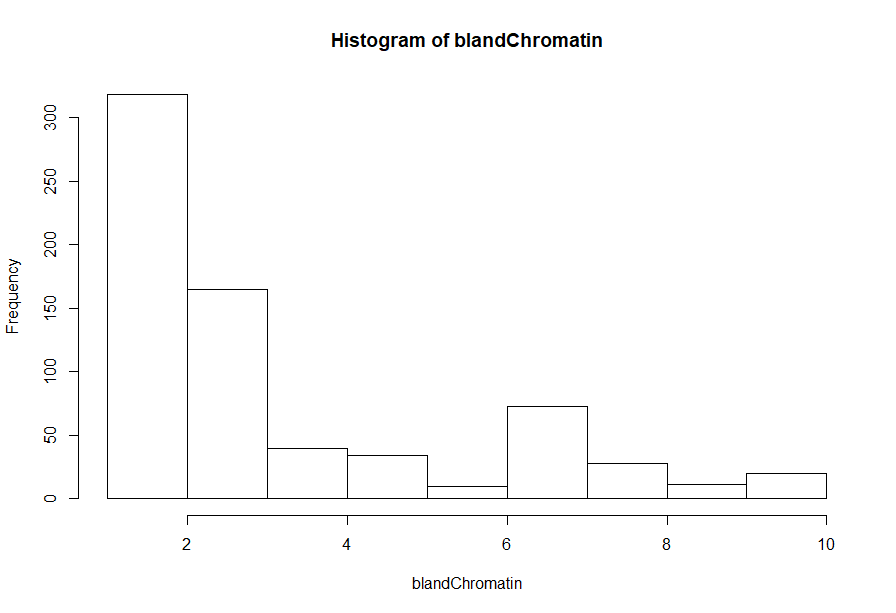
\includegraphics[width=\linewidth]{histv8.png}
  \caption{Bland Chromatin: 1 - 10}
\end{figure}
\begin{figure}
  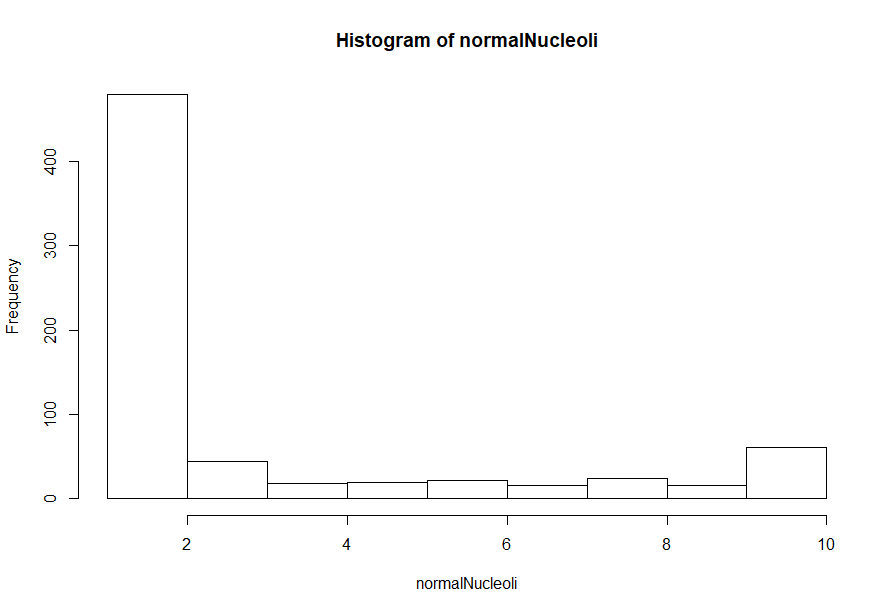
\includegraphics[width=\linewidth]{histv9.png}
  \caption{Normal Nucleoli: 1 - 10}
\end{figure}
\begin{figure}
  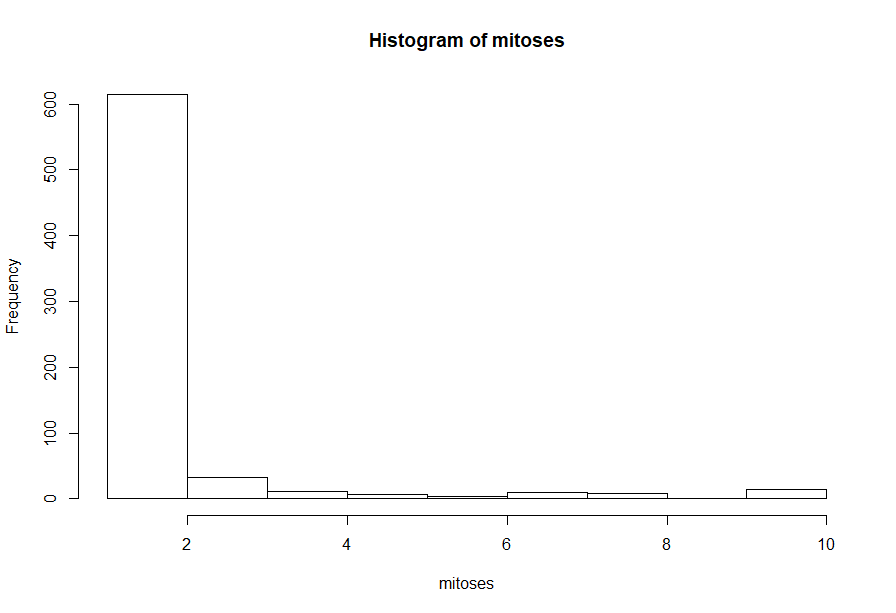
\includegraphics[width=\linewidth]{histv10.png}
  \caption{Mitoses: 1 - 10}
\end{figure}
\begin{figure}
  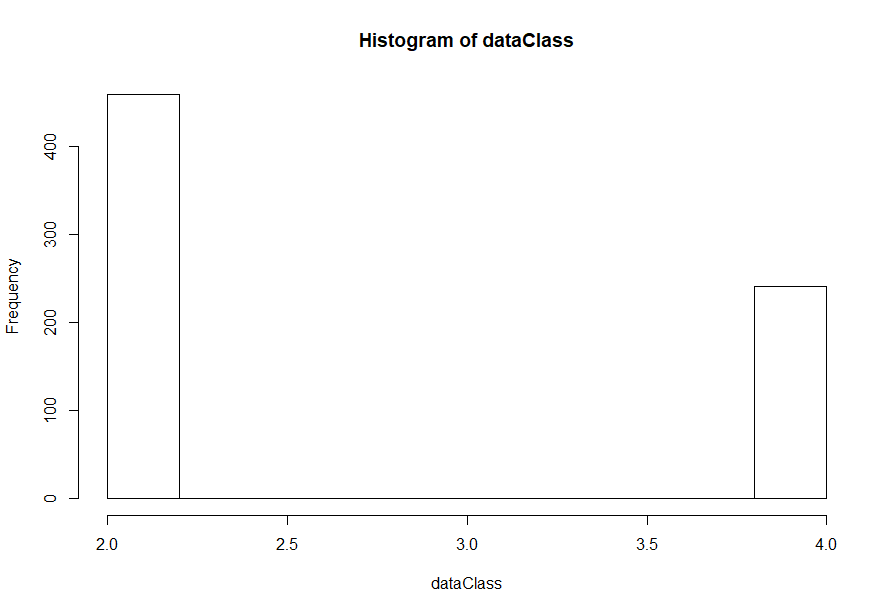
\includegraphics[width=\linewidth]{histv11.png}
  \caption{Class: (2 for benign, 4 for malignant)}
\end{figure}
\end{enumerate} 
\subsection{Discussion of simply removing tuples}
Quantify the affect of simply removing the tuples with unknown or missing values.  What is the cost in human capital?  \textbf{(20 points)}\\
When the missing value is removed, the data on the other attributes will also be removed, so we might lose a lot of information that is useful. Instead of removing missing value, we can use other algorithm, such as replace missing values with mean or median.
\end{homeworkProblem}


%----------------------------------------------------------------------------------------

\section*{What to Turn-in }
Please follow the syllabus guidelines in turning in your homework.  I am providing the \LaTeX{} of this document too. This homework is due Friday, Feb  9, 2018 10:00p.m. \textbf{OBSERVE THE  TIME}. Absolutely no homework will be accepted after that time. 
All the work should be your own.   Submit a .zip file that includes the files below. Name the .zip as \quotes{usename-section number}, i.e., hakurban-B365.
\begin{enumerate}
\item The *tex and *pdf of the written answers to this document.
\end{enumerate}

%----------------------------------------------------------------------------------------

\end{document}